\documentclass[aspectratio=169]{beamer}
\usepackage[utf8]{inputenc}
\usepackage{hyperref}
\usepackage{amsmath,amsfonts,amsthm,bm}
\usepackage{color}
\usepackage{graphicx} % Allows including images
\usepackage{subcaption}
\usepackage{booktabs} % Allows the use of \toprule, \midrule and \bottomrule in tables
\usepackage{tikz}
\usetikzlibrary{automata,positioning}
%\usepackage{pgfplots}
\usepackage{adjustbox}
\usepackage{listings}
\usepackage{courier}
\usepackage[version=4]{mhchem}
\usepackage{array}
\usepackage{modiagram}

\lstset{ %
  basicstyle=\scriptsize\ttfamily, % fonts that are used for the code
  breakatwhitespace=false,         % sets if automatic breaks should only happen at whitespace
  %breaklines=true,                 % sets automatic line breaking
  %captionpos=b,                    % sets the caption-position to bottom
  commentstyle=\color{gray}\textit,    % comment style
  keepspaces=true,                 % keeps spaces in text, useful for keeping indentation of code (possibly needs columns=flexible)
  keywordstyle=\color{blue},       % keyword style
  language=Python,                 % the language of the code
  %otherkeywords={*,...},          % if you want to add more keywords to the set
  rulecolor=\color{black},         % if not set, the frame-color may be changed on line-breaks within not-black text (e.g. comments (green here))
  showspaces=false,                % show spaces everywhere adding particular underscores; it overrides 'showstringspaces'
  showstringspaces=false,          % underline spaces within strings only
  showtabs=false,                  % show tabs within strings adding particular underscores
  stringstyle=\color{red}, % string literal style
  tabsize=4,	                   % sets default tabsize to 2 spaces
  columns=fixed                    % Using fixed column width (for e.g. nice alignment)
}

\hypersetup{
    colorlinks=true,
    linkcolor=red,
    filecolor=magenta,      
    urlcolor=red,
}

\DeclareMathOperator*{\argmax}{argmax}
\DeclareMathOperator*{\argmin}{argmin}
\let \vec \mathbf

\newcommand{\classname}{NANO266}
\newcommand{\classyear}{Fall 2024}
\mode<presentation> {
    \usetheme{CambridgeUS}
    \setbeamertemplate{footline}[text line]{%
      \parbox{\linewidth}{\vspace*{-8pt}\classname\hfill\classyear\hfill\insertpagenumber}}

    %\setbeamertemplate{footline}[page number]
    \setbeamertemplate{navigation symbols}{}
}


\title[\classname The Hartree Fock Approximation]{\classname~- Quantum Mechanical Modeling of Materials and Nanostructures\\The Hartree Fock Approximation}

\author{Shyue Ping Ong}
\institute[UCSD]{University of California, San Diego\\
\medskip
}
\date{\classyear} % Date, can be changed to a custom date

\begin{document}


\begin{frame}
    \titlepage % Print the title page as the first slide
\end{frame}

\begin{frame}{Stationary Schr\"odinger Equation}
\begin{eqnarray*}
    H\phi(\vec{r}) = E\phi(\vec{r}) 
\end{eqnarray*}
where

\begin{eqnarray*}
    H = -\sum_i \frac{\bar{h}^2}{2m_e}\nabla_i^2
    -\sum_k \frac{\bar{h}^2}{2m_k}\nabla_k^2
    -\sum_i\sum_k \frac{e^2Z_k}{r_{ik}}
    +\sum_i\sum_j \frac{e^2}{r_{ij}}
    +\sum_k\sum_l \frac{e^2Z_kZ_l}{r_{kl}}
\end{eqnarray*}
 \end{frame}

\begin{frame}{Switching to natural atomic units}
\begin{table}[]
    \centering
    \begin{tabular}{ccc}
        \textbf{Dimension} & \textbf{Unit} & \textbf{Symbol }\\
        \hline
        Mass & Electron rest mass & $m_e$\\
        Charge & Elementary Charge & $e$\\
        Action & Reduced Planck's constant & $\bar{h}$\\
        Electric constant & Coulomb force constant & $k_e$
    \end{tabular}
\end{table}

\begin{eqnarray*}
    H = -\sum_i \frac{1}{2}\nabla_i^2
    -\sum_k \frac{1}{2m_k}\nabla_k^2
    -\sum_i\sum_k \frac{Z_k}{r_{ik}}
    +\sum_i\sum_j \frac{1}{r_{ij}}
    +\sum_k\sum_l \frac{Z_kZ_l}{r_{kl}}
\end{eqnarray*}
    
\end{frame}

\begin{frame}{Recap: Variational Principle}

We can judge the quality of a guess wave functions by the energy – \textbf{the lower the energy, the better}. We may also use any arbitrary basis set to expand the guess wave function.

    \begin{eqnarray*}
    \frac{\int \phi^* H \phi d\vec{r}}{\int |\phi|^2 d\vec{r}} \geq E_0
    \end{eqnarray*}

How do we use this?
\end{frame}


\begin{frame}{Linear combination of atomic orbitals (LCAO)}

\begin{figure}
\begin{subfigure}{0.45\textwidth}
\begin{modiagram}
 \atom{left}{1s={;up}}
 \atom{right}{1s={;down}}
 \molecule{
    1sMO={;pair,up}
 }
\end{modiagram}
\caption{\ce{H2} molecule}
\end{subfigure}
\begin{subfigure}{0.45\textwidth}
    \includegraphics[width=\linewidth]{lectures/figures/2_atomic_orbitals.png}
    \caption{Source: http://orbitals.com}
    \end{subfigure}
\end{figure}
Express trial wave functions for molecular orbtial using atomic orbitals as a basis set.

\begin{equation*}
    \phi = \sum_i a_i \psi_i
\end{equation*}

\end{frame}

\begin{frame}{Secular equation}

\begin{columns}
    \column{0.5\textwidth}
\begin{eqnarray*}
    E & = &\frac{\int \sum_i a_i \psi_i^* H \sum_j a_j \psi_i d\vec{r}}{\int |\sum_i a_i \psi_i|^2 d\vec{r}}\\
    & = &\frac{\sum_{ij} a_i a_j \int \psi_i^* H \psi_j d\vec{r}}{\sum_{ij} a_i a_j \int \psi_i^* \psi_j d\vec{r}}\\
    & = &\frac{\sum_{ij} a_i a_j H_{ij}}{\sum_{ij} a_i a_j S_{ij} }\\
\end{eqnarray*}

$H_{ij}$: Resonance integral\\
$S_{ij}$: Overlap integral

    \column{0.5\textwidth}

Minimizing $E$ with respect to coeffients $a_i$,

\begin{eqnarray*}
    \frac{\partial E}{\partial a_k} & = & 0, \forall k \\
    \sum_i a_i (H_{ki} - E S_{ki}) & = & 0, \forall k
\end{eqnarray*}

In matrix form,
\begin{equation*}
\begin{pmatrix}
H_{11}-ES_{11} & ... & H_{1N}-ES_{1N}\\
... & ... & ...\\
H_{N1}-ES_{N1} & ... & H_{NN}-ES_{NN}\\
\end{pmatrix}
\begin{pmatrix}
a_1\\
...\\
a_N\\
\end{pmatrix}
= 0
\end{equation*}
\end{columns}
\end{frame}


\begin{frame}{Solving the Secular equation}

Solutions exist only if
\begin{equation*}
\begin{vmatrix}
H_{11}-ES_{11} & ... & H_{1N}-ES_{1N}\\
... & ... & ...\\
H_{N1}-ES_{N1} & ... & H_{NN}-ES_{NN}\\
\end{vmatrix}
= 0
\end{equation*}

Procedure:
\begin{enumerate}
    \item Select a set of $N$ basis functions.
    \item Determine all $N^2$ values of $H_{ij}$ and $S_{ij}$.
    \item Construct the secular determinant and determine the $N$ roots $E_i$.
    \item For each $E_i$, solve for the coefficients $a_i$.
\end{enumerate}
\end{frame}

\begin{frame}{Example: H\"uckel Theory, circa 1930}
\begin{columns}
    \column{0.5\textwidth}
    Basis set formed by C 2$p$ orbitals\\
    Overlap matrix given by
    \begin{equation*}
        S_{ij} = \delta_{ij}
    \end{equation*}
    $H_{ii}$ = Ionization potential of methyl radical, $\alpha$\\
    $H_{ij}$ for nearest neighbors from experiments, $\beta$, and 0 for non-nearest neighbors.
    \begin{equation*}
    \begin{vmatrix}
    \alpha-E & \beta & 0\\
    \beta & \alpha-E & \beta\\
    \beta & \beta & \alpha-E\\
    \end{vmatrix}
    = 0
    \end{equation*}
    \column{0.5\textwidth}
    \begin{figure}
        \centering
        \includegraphics[width=\linewidth]{lectures/figures/2_alkene.png}
    \end{figure}
\end{columns}
\end{frame}


\begin{frame}{Born-Oppenheimer Approximation}
Heavier nuclei move much more slowly than electrons $\implies$ Electronic relaxation is ``instantaneous'' with respect to nuclear motion.

Electronic Schr\"odinger Equation:
\begin{equation*}
    H_{el} \chi_{el}(\vec{r_i}; \vec{R_k}) = E_{el}\chi_{el}(\vec{r_i}; \vec{R_k})
\end{equation*}

where $\vec{r_i}$ represents the electronic coordinates and $\vec{R_k}$ represents the nuclear coordinates, which are fixed.

\begin{equation*}
    H_{el} = -\sum_i \frac{1}{2}\nabla_i^2
    -\sum_i\sum_k \frac{Z_k}{r_{ik}}
    +\sum_i\sum_j \frac{1}{r_{ij}}
\end{equation*}

\end{frame}


\begin{frame}{Effective potential assumption}

The electronic Schr"odinger equation can be greatly simplified using a mean-field assumption to break down the many-electron Hamitonian as a sum of one-electron Hamiltonians:

KE and nuclear attraction terms are trivially separable:
\begin{equation*}
    -\sum_i \frac{1}{2}\nabla_i^2
    -\sum_i\sum_k \frac{Z_k}{r_{ik}}
    = \sum_i \left[ - \frac{1}{2}\nabla_i^2
    -\sum_k \frac{Z_k}{r_{ik}}\right]
\end{equation*}

To include electron-electron repulsion, assume that each electron sees an ``effective'' potential from the other electrons:

\begin{equation*}
    \sum_i\sum_j \frac{1}{r_{ij}}
    = \sum_i \sum_{i \neq j} \int \frac{\rho}{r_{ij}} d \vec{r}
\end{equation*}

\end{frame}

\begin{frame}{Hartree-Product Wave Functions}

\begin{eqnarray*}
    H_{el} = \sum_i h_i, \mbox{where}~h_i = - \frac{1}{2}\nabla_i^2
    -\sum_k \frac{Z_k}{r_{ik}} + \sum_{i \neq j} \int \frac{\rho}{r_{ij}} d \vec{r}
\end{eqnarray*}

Because $H_{el}$ is separable, 
\begin{eqnarray*}
    \psi_{HP} & = & \prod_i \phi_i \\
    H_{el} \psi_{HP} & = & \sum_i h_i \prod_i \phi_i \\
                    & = & \sum_i \varepsilon_i \prod_i \phi_i \\
\end{eqnarray*}

\end{frame}


\begin{frame}{Hartree Self-Consistent Field (SCF) Approach}
\begin{figure}
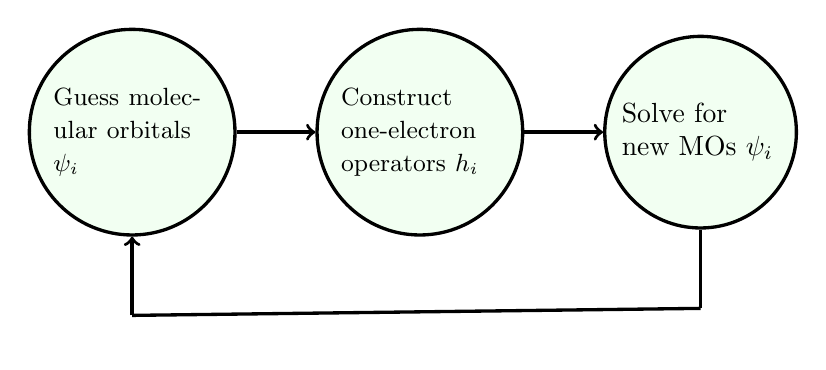
\begin{tikzpicture}
[
roundnode/.style={circle, draw=black, fill=green!5, very thick, radius=2cm},
invisiblenode/.style={circle,radius=0},
node distance=1cm,
]
%Nodes

\node[roundnode] (node1) [text width=2cm]{\small{Guess molecular orbitals $\psi_i$}};
\node[roundnode] (node2) [right=of node1, text width=2cm] {\small{Construct one-electron operators $h_i$}};
\node[roundnode] (node3) [right=of node2, text width=2cm] {Solve for new MOs $\psi_i$};
\node[invisiblenode] (node4) [below=of node3] {};
\node[invisiblenode] (node5) [below=of node1] {};

%Lines
\draw[->, very thick] (node1.east) -- (node2.west);
\draw[->, very thick] (node2.east) -- (node3.west);
\draw[-, very thick] (node3.south) -- (node4.north);
\draw[-, very thick] (node4.north) -- (node5.north);
\draw[->, very thick] (node5.north) -- (node1.south);
\end{tikzpicture}
\end{figure}
Iterate until convergence.
\begin{eqnarray*}
    E = \sum_i \varepsilon_i - \frac{1}{2} \int \int \frac{\left|\psi_i\right|^2\left|\psi_j\right|^2}{r_{ij}} d \vec{r_i} d \vec{r_j} ~(\mbox{\textcolor{red}{Why?}})
\end{eqnarray*}

\end{frame}

\begin{frame}{Pauli Exclusion Principle}
Two identical fermions (spin 1/2 particles) cannot occupy the same quantum state simultaneously $\implies$ Wave function has to be anti-symmetric. For two electron system:
\begin{eqnarray*}
    \psi_{SD} & = & \frac{1}{\sqrt{2}}\left[ \psi_a(1) \alpha(1) \psi_b(2) \alpha(2) - \psi_a(2) \alpha(2) \psi_b(1) \alpha(1)\right] \\
    & = & \frac{1}{\sqrt{2}} \begin{vmatrix}
        \psi_a(1) \alpha(1) & \psi_b(1) \alpha(1) \\
        \psi_a(2) \alpha(2) & \psi_b(2) \alpha(2)
    \end{vmatrix} 
\end{eqnarray*}

where $\alpha$ is the electron spin eigenfunction. For many electrons,
\begin{eqnarray*}
    \psi_{SD} & = & \frac{1}{\sqrt{N!}} \begin{vmatrix}
        \chi_1(1) & ... & \chi_N(1) \\
        ... & ... & ...\\
        \chi_1(N) & ... & \chi_N(N)
    \end{vmatrix} 
\end{eqnarray*}

where $\chi_k$ are the spin orbitals.
\end{frame}


\begin{frame}{The Hartree-Fock (HF) SCF Method}

\begin{equation*}
    f_i = - \frac{1}{2}\nabla_i^2
    -\sum_k \frac{Z_k}{r_{ik}} + V_i^{HF}(j)
\end{equation*}

\begin{alertblock}{HF Secular Equation}
    \begin{equation*}
\begin{vmatrix}
F_{11}-ES_{11} & ... & F_{1N}-ES_{1N}\\
... & ... & ...\\
F_{N1}-ES_{N1} & ... & F_{NN}-ES_{NN}\\
\end{vmatrix}
= 0
\end{equation*}
\end{alertblock}

    \begin{equation*}
F_{\mu\upsilon} = \langle \mu | - \frac{1}{2}\nabla_i^2 | \upsilon \rangle
    -\sum_k Z_k \langle \mu |\frac{1}{r_{ik}}\upsilon \rangle + \sum_{\lambda \sigma} [ (\mu\upsilon| \lambda\sigma) - \frac{1}{2} (\mu\lambda| \upsilon\sigma)]
\end{equation*}

\end{frame}

\begin{frame}{HF SCF Flowchart}
\begin{figure}
    \centering
    \includegraphics[width=0.35\linewidth]{lectures/figures/2_HF_SCF_Flowchart.png}

\end{figure}
    
\end{frame}

\begin{frame}{Limitations of HF}
Fock operators are one-electron $\implies$ All electron correlation, other than exchange, is ignored.

\begin{alertblock}{Definition of electron correlation}
\begin{equation*}
    E_{corr} = E_{exact} - E_{HF} 
\end{equation*}
\end{alertblock}

Four-index integrals lead to $N^4$ scaling with respect to the size of the base set.

\end{frame}

\begin{frame}{Basis Sets}

\begin{itemize}
    \item Set of mathematical functions used to construct the wave function.
    \item In theory, HF limit is achieved by an infinite basis set.
    \item In practice, use finite basis sets that can approach HF limit as efficiently as possible
\end{itemize}

\end{frame}


\begin{frame}{Contracted Gaussian Functions}

\begin{columns}
    \column{0.5\textwidth}
Slater-type orbitals (STO) with $e^{-r}$ radial decay cannot be analytically integrated.\newline
\newline
\textbf{Solution: }Use linear combination of Gaussian-type orbitals (GTOs) with $e^{-r^2}$ radial decay to approximate STOs.\newline
\newline
STO-3G:
\begin{itemize}
\item STO approximated by 3 GTOs
\item Known as single-$\zeta$ or minimal basis set. 
\end{itemize}

    \column{0.5\textwidth}
    \begin{figure}
        \centering
        \includegraphics[width=\linewidth]{lectures/figures/2_STO.png}
    \end{figure}
\end{columns}

\end{frame}


\begin{frame}{Multiple $\zeta$ and Split-Valence Basis Sets}
\textbf{Multiple-$\zeta$}
\begin{itemize}
    \item Adding more basis functions per atomic orbital
    \item Examples: cc-pCVDZ, cc-pCVTZ, or correlation-consistent polarized Core and Valence (Double/Triple/etc.) Zeta
\end{itemize}

\textbf{Split-valence or Valence-Multiple-$\zeta$}
\begin{itemize}
    \item Still represent core orbitals with single, contracted basis functions. 
    \item Valence orbitals are split into many functions (Why?)
    \item Examples: 3-21G, 6-31G, 6-311G
    \item Notation: X-YZg, where X = no. of primitive Gaussians for each core orbitals, Y and Z = no. of primitive Gaussians for valence orbitals. 
\end{itemize}

\end{frame}

\begin{frame}{Polarization and Diffuse Functions}
    \textbf{Polarization functions}
    \begin{itemize}
        \item Description of some MOs requires more flexibility than provided by AOs, e.g., \ce{NH3} is predicted to be planar if using just $s$ and $p$ functions.
        \item Additional basis functions of one quantum number of higher angular momentum than valence, e.g., first row $\rightarrow$ $d$ orbitals.
        \item Notation: 6-31G(d), 6-31(2d,p) [2d functions for heavy atoms, additional p for H]
    \end{itemize}

\textbf{Diffuse functions}
\begin{itemize}
    \item Highest energy MOs of anions, highly excited states tend to be more diffuse.
    \item Augment standard basis sets with diffuse functions.
    \item Notation: 6-31+G, 6-311++G(3df, 2pd), aug-cc-pCVDZ
\end{itemize}

\end{frame}

\begin{frame}{Effective Core Potentials}
    Heavy atoms have many electrons $\implies$ Intractable to model all of them, even with a minimal basis set.\newline
\newline
However, most of the electrons are in the core.\newline
\newline
\textbf{Solution:} Replace core electrons with analytical functions (effective core potentials or ECPs) that represent combined nuclear-electronic core to the remaining electrons.\newline
\newline
\textbf{Key selection decision:} How many electrons to include in the core?

\end{frame}


\begin{frame}{Open-shell vs Closed-shell}
Restricted HF (RHF): Closed-shell systems, i.e., no unpaired electrons.\newline
\newline
Restricted open-shell HF (ROHF): Use RHF formalism, but with density matrix for singly occupied orbitals not multiplied by a factor of 2. Wave functions are eigenfunctions of S2 But fails to account for spin polarization in doubly occupied orbitals.\newline
\newline
Unrestricted HF (UHF): Includes spin polarization, but wave functions are not eigenfunctions of S2, i.e., spin contamination

\end{frame}

\begin{frame}{Accuracy of HF}

Energetics
\begin{itemize}
    \item In general, extremely poor; correlation is extremely important in chemical bonding!
    \item Protonation energies are typically ok (no electrons in \ce{H+})
    \item Koopman's Theorem: First IE is equal to the negative of the orbital energy of the HOMO
\end{itemize}

Geometry
\begin{itemize}
    \item Typically relatively good ground state structures with basis sets of modest siz.
    \item But transition states (with partial bonding) can be problematic, as well as some pathological systems.
\end{itemize}

\end{frame}

\begin{frame}{Computational speed}
Formal $N^4$ scaling.

But in reality, speedups can be achieved through:
\begin{itemize}
    \item Symmetry
    \item Estimating upper bounds to four-index integrals
    \item Fast multipole and linear exchange integral computations
\end{itemize}

For practical geometry optimizations, frequently helps to first compute geometry with a smaller basis set to provide a better initial geometry and a guess for the Hessian matrix.
    
\end{frame}


\begin{frame}[allowframebreaks]{Bibliography}
    \bibliographystyle{unsrt}
    \bibliography{refs}
\end{frame}



\begin{frame}
    \Huge{\centerline{The End}}
\end{frame}

\end{document}

